\documentclass[11pt]{article}
% decent example of doing mathematics and proofs in LaTeX.
% An Incredible degree of information can be found at
% http://en.wikibooks.org/wiki/LaTeX/Mathematics

% Use wide margins, but not quite so wide as fullpage.sty
\marginparwidth 0.5in 
\oddsidemargin 0.25in 
\evensidemargin 0.25in 
\marginparsep 0.25in
\topmargin 0.25in 
\textwidth 6in \textheight 8 in
% That's about enough definitions
\usepackage[usenames, dvipsnames]{color}
\usepackage{graphicx}
\graphicspath{ {report-images/} }
\usepackage[colorlinks=true]{hyperref}

\usepackage{array}
\usepackage{rotating}
\newcolumntype{L}[1]{>{\raggedright\let\newline\\\arraybackslash\hspace{0pt}}m{#1}}
\newcolumntype{C}[1]{>{\centering\let\newline\\\arraybackslash\hspace{0pt}}m{#1}}
\newcolumntype{R}[1]{>{\raggedleft\let\newline\\\arraybackslash\hspace{0pt}}m{#1}}

\definecolor{mypink1}{rgb}{0.858, 0.188, 0.478}
\definecolor{mypink2}{RGB}{219, 48, 122}
\definecolor{mypink3}{cmyk}{0, 0.7808, 0.4429, 0.1412}
\definecolor{mygray}{gray}{0.6}

\usepackage{listings}
\usepackage{color}
\usepackage{float}

\definecolor{dkgreen}{rgb}{0,0.6,0}
\definecolor{gray}{rgb}{0.5,0.5,0.5}
\definecolor{mauve}{rgb}{0.58,0,0.82}

\lstset{frame=tb,
	language=Java,
	aboveskip=3mm,
	belowskip=3mm,
	showstringspaces=false,
	columns=flexible,
	basicstyle={\small\ttfamily},
	numbers=none,
	numberstyle=\tiny\color{gray},
	keywordstyle=\color{blue},
	commentstyle=\color{dkgreen},
	stringstyle=\color{mauve},
	breaklines=true,
	breakatwhitespace=true,
	tabsize=3
}

\lstdefinestyle{SQL}{
	language={SQL},basicstyle=\ttfamily, 
	moredelim=**[is][\btHL]{`}{`},
	moredelim=**[is][{\btHL[fill=green!30,draw=red,dashed,thin]}]{@}{@},
}

\usepackage{amsmath}
\usepackage{upgreek}
\usepackage{xepersian}
\settextfont{XB Niloofar}
\setdigitfont{XB Niloofar}




\begin{document}
	\author{\textcolor{mauve}{افرا امینی، پری‌شاد بهنام قادر، حنانه اکرمی}}
	\title{گزارش فاز سوم - معماری و شمای پایگاه داده}
	\maketitle
	\section{تکنولوژی‌های استفاده شده}
	پروژه بنگاه کمک به کودکان در چهارچوب (framework) Django پیاده‌سازی شده و تکمیل خواهد شد. پایگاه داده مورد استفاده postgresql است. هم‌چنین برای طراحی رابط کاربری به منظور زیبایی و سادگی طراحی از Bootstrap بهره می‌بریم. در شکل زیر معماری کلی درنظر گرفته شده را می‌بینید:
	\begin{figure}[H]
	\centering
	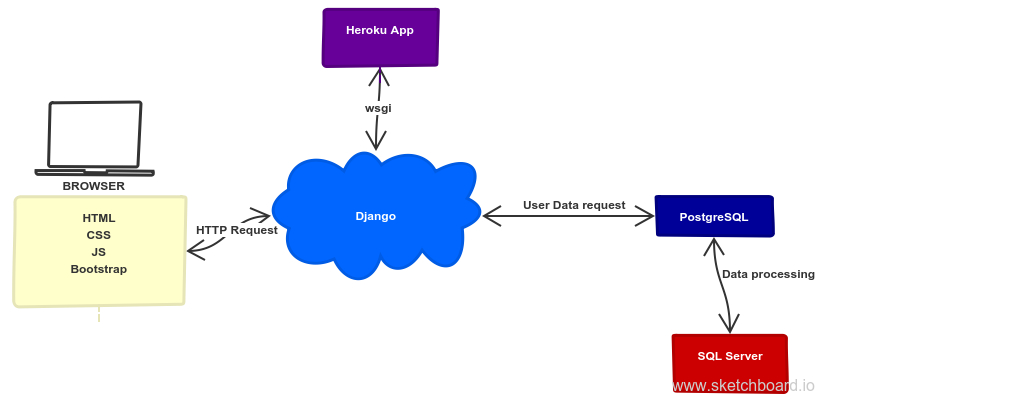
\includegraphics[width=15 cm]{memari}
	\caption{معماری درنظر گرفته شده}
	\end{figure}	
	\section{شمای پایگاه داده}
	در شکل زیر که در پروژه هم پیوست شده‌است شمای مدل‌های طراحی شده برای پایگاه داده را می‌بینید که حاوی نیاز‌های داده‌ای انواع کاربران(مددجویان، مددکاران، همیاران و مدیر) می‌باشد.\\
	کاربر در این سامانه دارای مشخصاتی کلی همچون نام و نام‌خانوادگی می‌باشد. کاربران خاص‌تر همگی نوعی از کاربر اصلی هستند(رابطه \lr{is a} ) که به فراخور نیاز، دارای مشخصات و روابطی با دیگر موجودیت‌ها می‌باشند.\\
	برخی از نیاز‌های داده‌ای کاربر به اختصار شرح داده می‌شود:
	\begin{itemize}
		\item مددجو می‌تواند برای همیار نامه ارسال کند.
		\item مددجو تعدادی نیاز دارد.
		\item همیار می‌تواند یک مددجو را تحت تکفل خود قرار دهد.
		\item همیار می‌تواند به مددجوی تحت تکفل خود پرداخت کند.
		\item همیار می‌تواند به مددکار نامه ارسال کند.
	\end{itemize}
	تمامی موارد بالا داده‌هایی تولید می‌کنند که لازم است در پایگاه داده ذخیره شود. در شکل صفحه بعد جداول پایگاه داده و ارتباط آن‌ها را با جزئیات می‌بینید.
	\newpage
	\begin{sidewaysfigure}[ht]
	\centering
	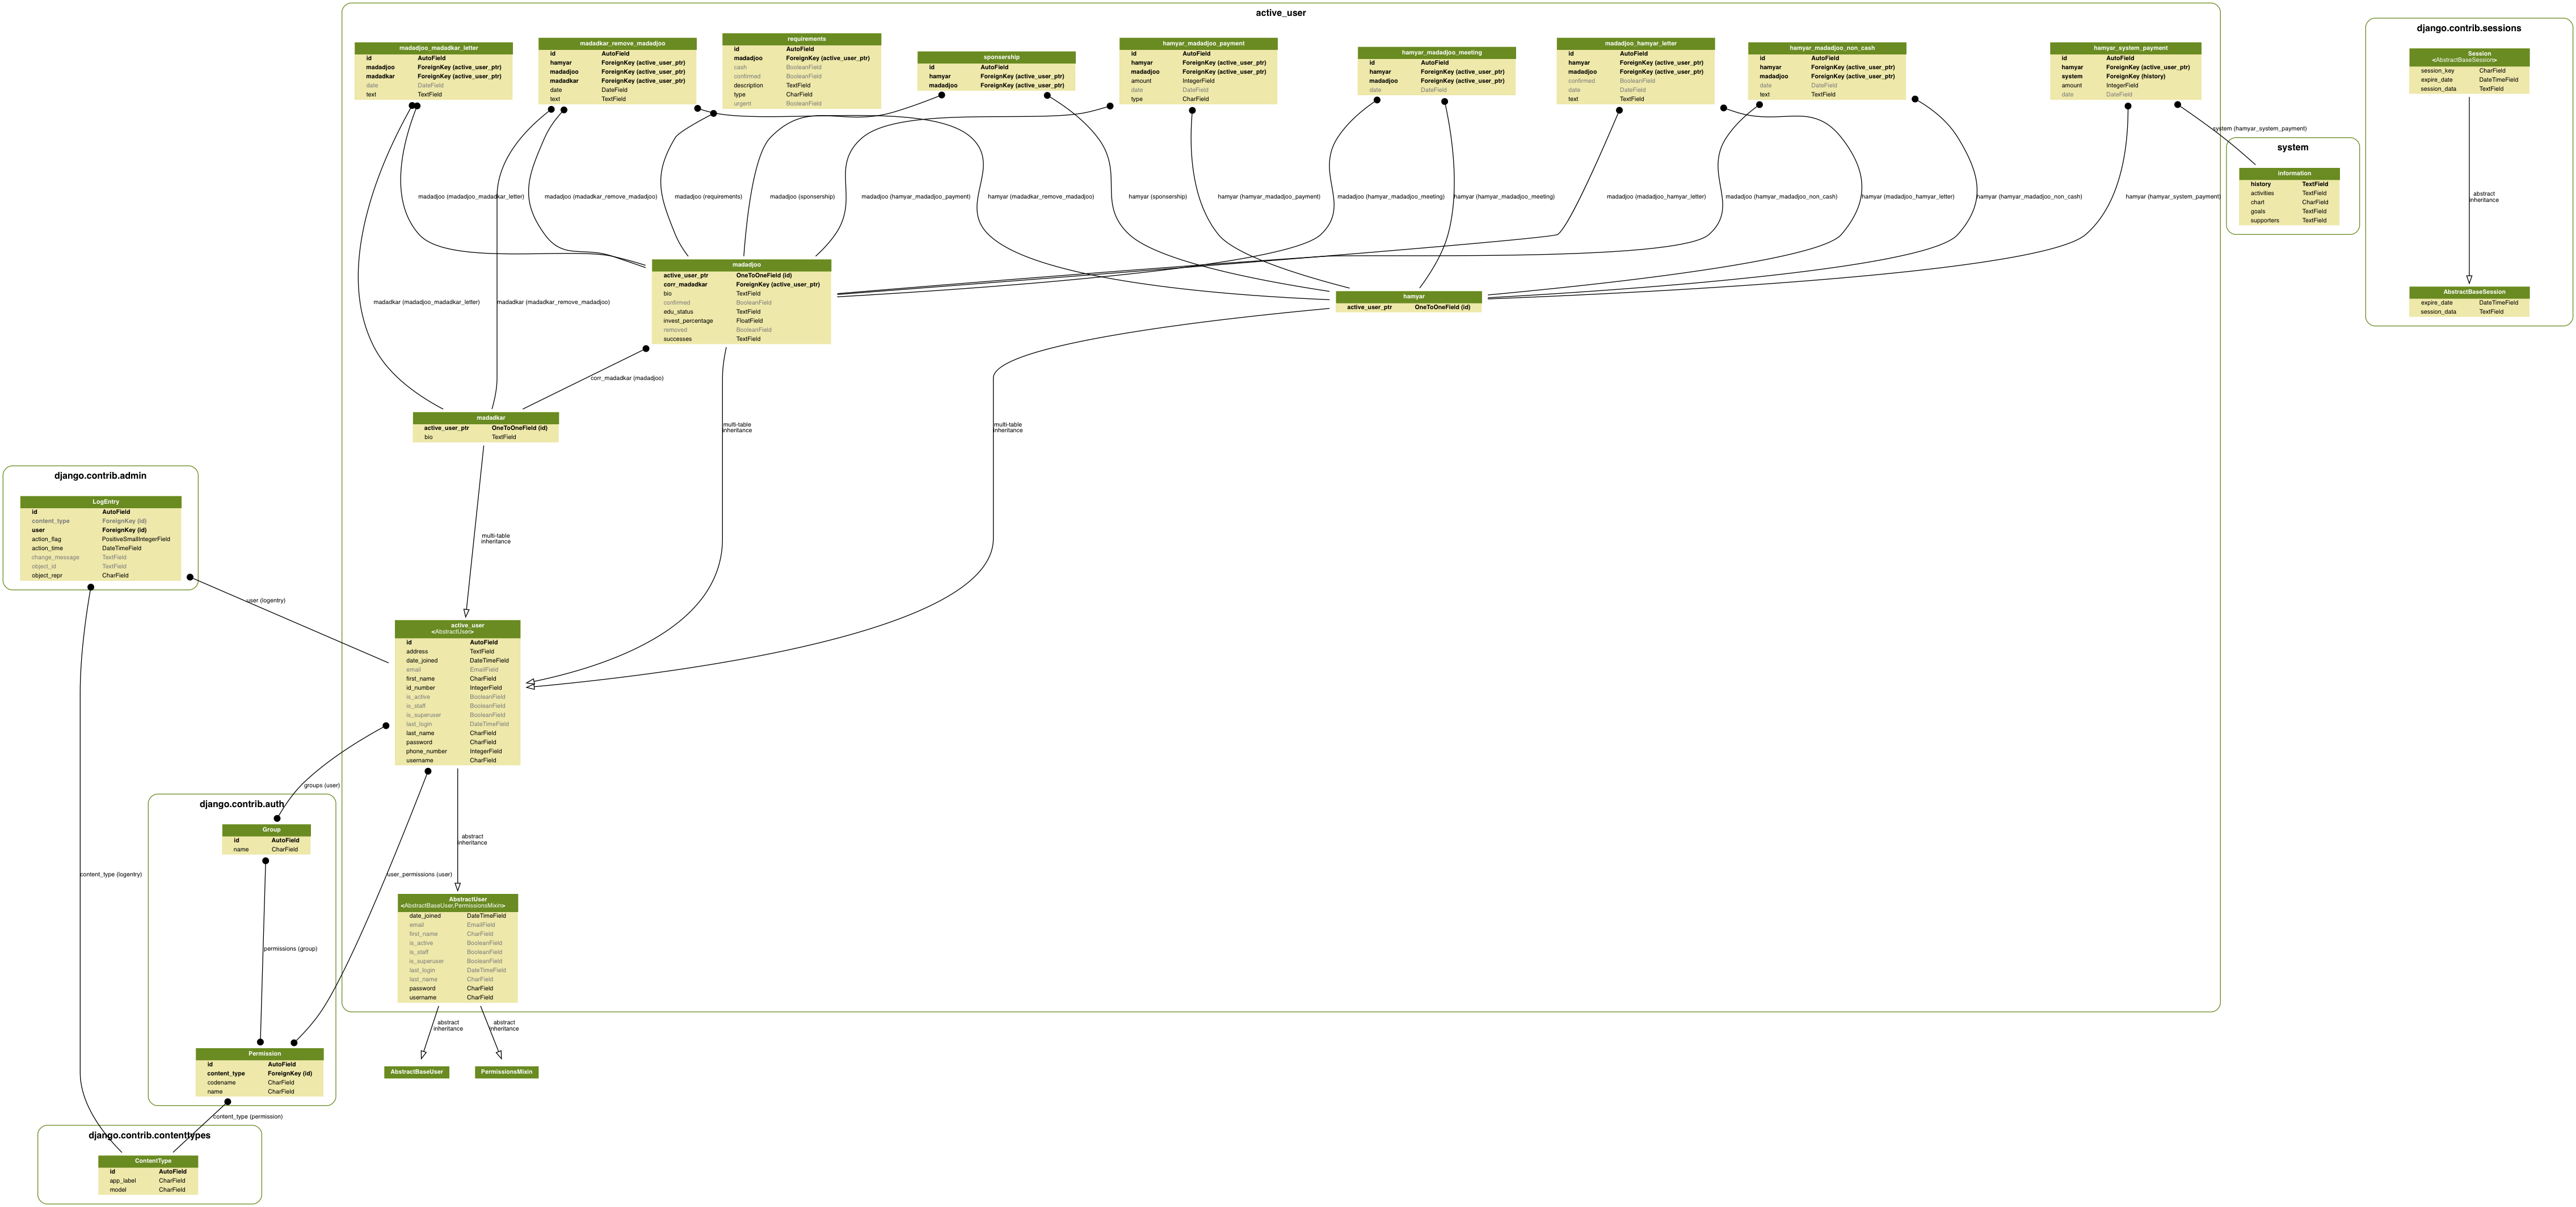
\includegraphics[width=\textwidth]{ChildF_visualized.png}
	\caption{شمای پایگاه داده}
	\end{sidewaysfigure}	
	
\end{document}


